\begin{figure}[ht]
\ffigbox
	{\begin{subfigure}[b]{0.48\linewidth}
		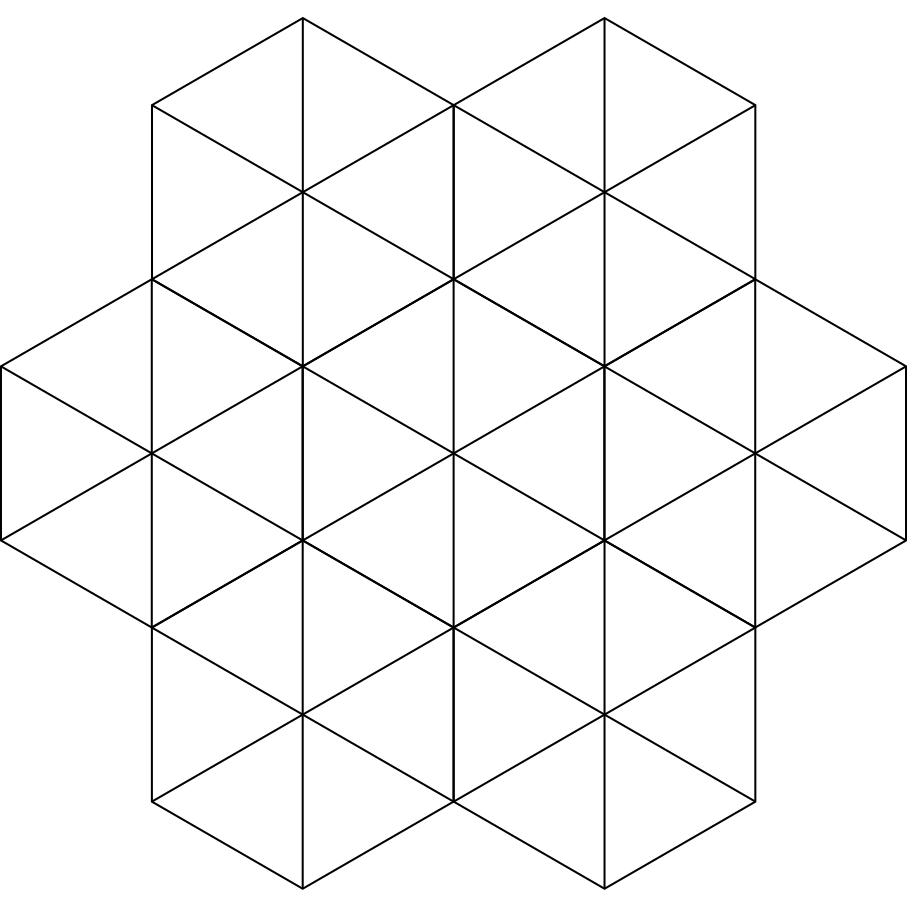
\includegraphics[width=1.0\linewidth,height=0.3\textheight,keepaspectratio]{data/synthetic_meshes/hexagonal_tessellation_Dirac_delta_1_v31_f42_wireframe.png}
		\caption{Hex v31\_f42 wireframe}\label{fig:hex.a}
	\end{subfigure}
	\begin{subfigure}[b]{0.48\linewidth}
		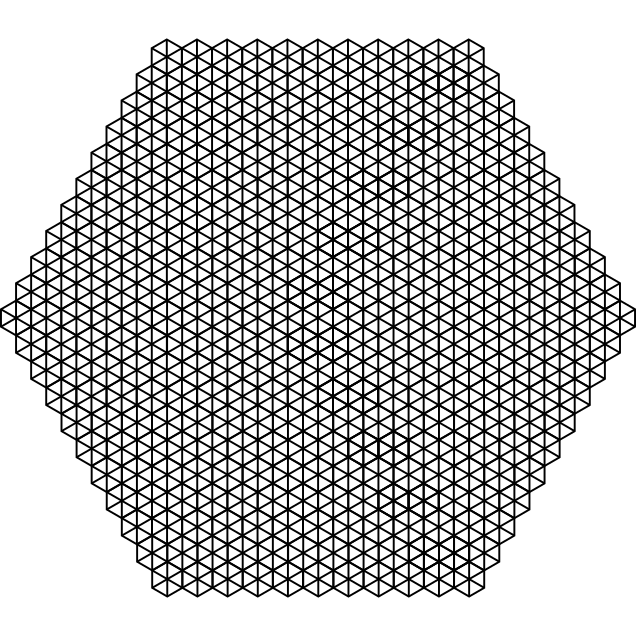
\includegraphics[width=1.0\linewidth,height=0.3\textheight,keepaspectratio]{data/synthetic_meshes/hexagonal_tessellation_Dirac_delta_10_v1057_f1986_wireframe.png}
		\caption{Hex v1057\_f1986 wireframe}\label{fig:hex.b}
	\end{subfigure}

	\bigskip
	\begin{subfigure}[b]{0.48\linewidth}
		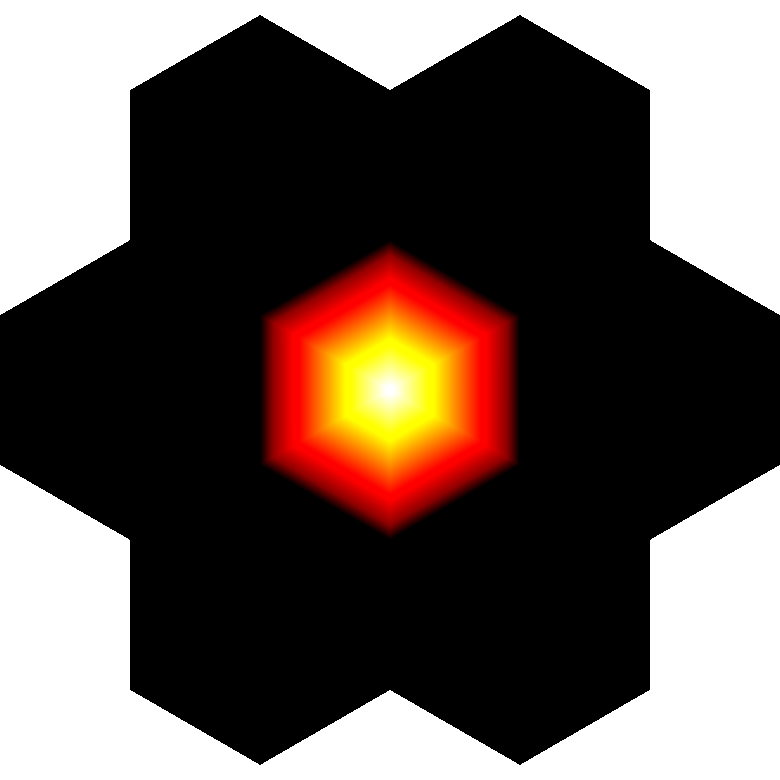
\includegraphics[width=1.0\linewidth,height=0.3\textheight,keepaspectratio]{data/synthetic_meshes/hexagonal_tessellation_Dirac_delta_1_v31_f42_funcvals_0iter_crop.png}
		\caption{Hex v31\_f42 iter 0}\label{fig:hex.c}
	\end{subfigure}
	\begin{subfigure}[b]{0.48\linewidth}
		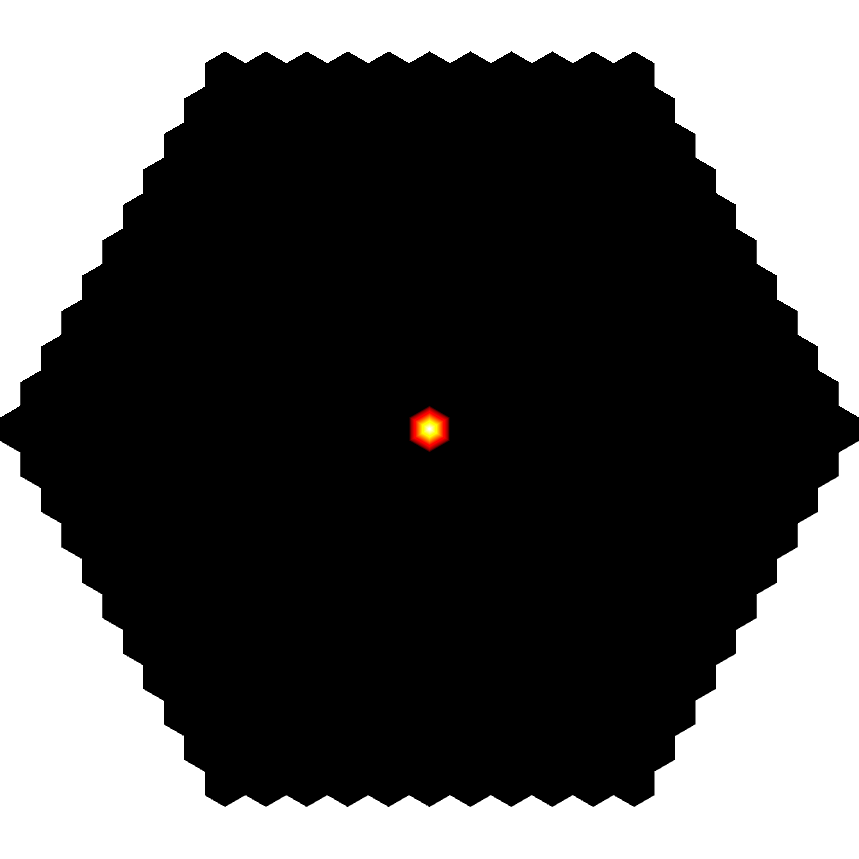
\includegraphics[width=1.0\linewidth,height=0.3\textheight,keepaspectratio]{data/synthetic_meshes/hexagonal_tessellation_Dirac_delta_10_v1057_f1986_funcvals_0iter_crop.png}
		\caption{Hex v1057\_f1986 iter 0}\label{fig:hex.d}
	\end{subfigure}

	\bigskip
	\begin{subfigure}[b]{0.48\linewidth}
		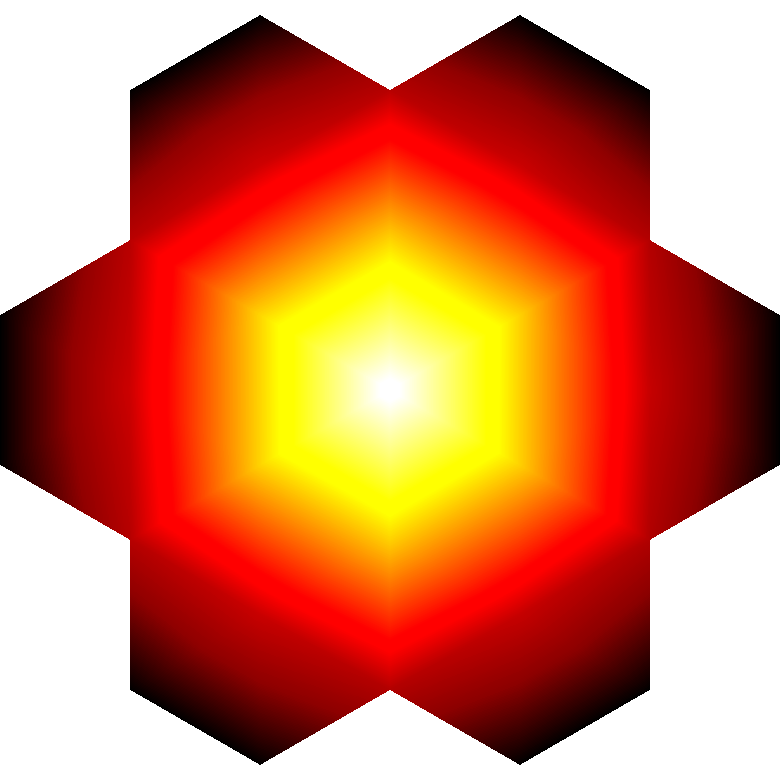
\includegraphics[width=1.0\linewidth,height=0.3\textheight,keepaspectratio]{data/synthetic_meshes/hexagonal_tessellation_Dirac_delta_1_v31_f42_funcvals_2iter_crop.png}
		\caption{Hex v31\_f42 iter 2}\label{fig:hex.e}
	\end{subfigure}
	\begin{subfigure}[b]{0.48\linewidth}
		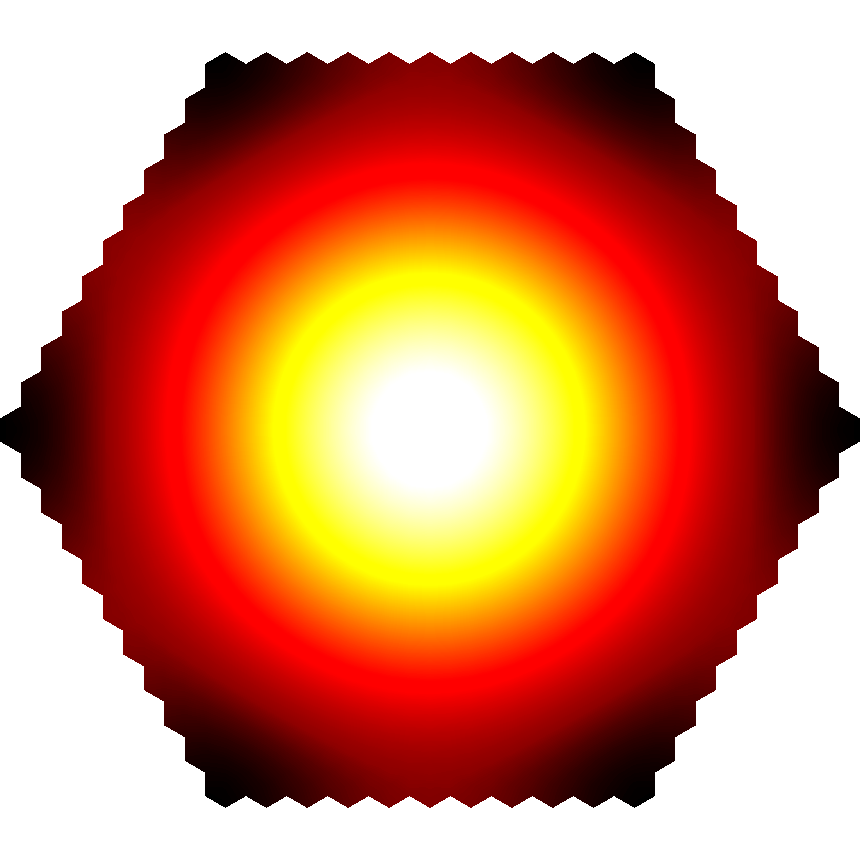
\includegraphics[width=1.0\linewidth,height=0.3\textheight,keepaspectratio]{data/synthetic_meshes/hexagonal_tessellation_Dirac_delta_10_v1057_f1986_funcvals_200iter_crop.png}
		\caption{Hex v1057\_f1986 iter 200}\label{fig:hex.f}
	\end{subfigure}}
	{\caption[Synthetic Hexagonal Tessellations, Dirac delta function]{A synthetic hexagonal tessellation, subdivided by triangles, with a Dirac delta function applied: (a) v31 f42 wireframe (b) v1057 f1986 wireframe (c) v31 f42 colored by function value before filter (d) v1057 f1986 colored by function value before filter (e) v31 f42 colored by function value after 2 iterations (e) v1057 f1986 colored by function value after 200 iterations.
% All using the colorramp "Hot (improved)"~\cite[p.~???]{Brewer2003}~\cite[p.~19]{Giga17}, visualized using GigaMesh~\cite{Mara10}, exported as png after disabling the background grid [f7], maximizing the window, disabling screenshot cropping, as well as rejecting tiled rendering, finally cropping to content in GIMP.
	}\label{fig:hex}}
\end{figure}
\todoCitation{}
